\chapter{Implementation}
\label{chapter: Implementation}
This chapter describes the implementation process of the automated feedback system and details on how the services and components of the project were implemented. It also provides diagrams of class diagrams, sequence diagrams, etc that help reader understand the system. It also explains the language, libraries, folders, and resources used in the application. Moreover, this chapter also provides an overview of how the feedback system is structured and how it works.
\newline
In the first section, the project structure is briefly explained, and graphical representations are provided. In the next step, the project components are analyzed and demonstrated using diagrams, followed by system flow diagrams.

\section{Project Structure}
The project structure for the feedback system is organized in order to make it easier to understand. Java packages are a way of organizing and managing related classes, interfaces, subclasses, exceptions, errors, and enums. This organized project structure makes it easy to locate the various components necessary for generating feedback on programming assignments with mutation testing. The components of the feedback system are divided into packages that are further subdivided and located in the sre/main/java. Additionally, there is also a test package that contains unit tests for each of the main packages in order to ensure that all functionality works as expected. \par

Java provides some built-in packages which we can use but we can also create our own (user-defined) packages by defining a directory with the same name as the package and placing classes inside it. The advantages of using Java Packages are that they make easy searching or locating of classes and interfaces; avoid naming conflicts; implement data encapsulation (or data-hiding); provide controlled access; allow for the reuse of classes contained in other packages, and uniquely compare classes in other packages. There are two types of packages in Java: Java API packages or built-in packages, which provide a large number of classes grouped into different packages based on a particular functionality, and user-defined packages which are created by the user.
\newpage
\begin{figure}[h!]
	\centering
\includegraphics[width=0.60\linewidth]{content/fig2.jpg}
% 	\includegraphics[scale=0.45]{content/fig2.jpg}
	\caption{Project structure}
	\label{fig:f12}
 \end{figure}

\subsection{Technologies and Tools used}
Technologies that are used in this project include:\\
intellij/eclipse sts, Java version 17, Maven, JUnit, PiTest, JSoup HTML Parser, Commons-IO, Zip4j, EclEmma, Log4j and Dropbox. \\
All the dependencies can be found in the “pom.xml” file.
\newline A Project Object Model (POM) is the core unit of Maven's build system. It is an XML document that contains information about the project, such as its configuration details, and provides default values for most projects. POMs are used by Maven to construct a project's overall build process, allowing developers to easily manage dependencies, build processes, and other aspects of the project. For the vast majority of projects, it comes with default settings.
\begin{itemize}
\item Java 17: As the newest long-term support (LTS) release for Java under its six-monthly release cycle, Java 17 is the latest release under that cycle. It was developed in collaboration with Oracle engineers as well as the entire Java community via the OpenJDK Community and the Java Community Process (JCP).
\item JUnit: As the name implies, JUnit is a framework for unit testing for the Java programming language. The JUnit framework is one of a family of unit testing frameworks that are collectively known as xUnit that originated with SUnit, and has played a very important role in the development of test-driven development. When Junit is compiled, it is linked as a JAR file and it is included in the build process.
\item PITEST: PITEST is a state-of-the-art mutation testing system that provides Java and the JVM with standard coverage for any changes made during development. This tool has a fast, scalable configuration, and it integrates well with modern tools for testing and building.
\item Mutation testing: The purpose of mutation testing is to improve the adequacy of tests and to uncover defects in a program by testing it against a range of different mutations. This is based on the idea that the production code is going to be changed dynamically and, as a result, the tests will fail.
\item Jsoup: This open-source Java library is designed to parse, extract, and manipulate data stored in HTML files.
\item Commons-IO: This is a collection of utilities for developing IO functionality as a part of Apache Commons IO. Among the six main areas in this package, there are six main groups: io - This package defines utility classes for working with streams, readers, writers, and files. File Comparator - This package provides different implementations of File Comparators for use with various file types.
\item Zip4j: This is the most complete Java library for zip files or streams. It also supports zip encryption.
\item Maven project manager tool. The Apache Group created the well-known open-source build tool Maven to create, publish, and distribute various projects simultaneously for improved project management. It is a tool that allows programmers to create and document the dynamic framework.
\item Log4j: It is a component of the Apache Software Foundation's Apache Logging Services project written by Ceki Gülcü.  
\end{itemize}

\newpage
\subsection{Architecture}
\subsubsection{Dropbox}
The feedback system uses Dropbox to store project files that have been submitted by students. Dropbox has four main folders. They include Submitted Project, the Project Success, projects processing and the Project Failure.
\begin{itemize}
\item Submitted Project: This folder contains projects that have been submitted by students.
\item Project Success: This folder contains project-passed Junit test and PiTest. Rclone moves these projects from the Local Server to the Project Failure folder.
\item Project Failure: This folder contains projects that have not passed the Junit test and PiTest. Rclone moves these projects from the Local Server to the Project Failure folder.
\item projects processing: this folder contains projects for processing.  
\end{itemize}
\subsubsection{Local Server}
This is a server where Feedback-Application is deployed and Rclone Program is installed. The Server has three parts that include: Folder directories, Rclone, and Feedback-App.
\subsubsection{Folder Directories}
The Local Server has four folder directories, which include Submitted Project, Project Processing, Project Success, and Project Failure.
\begin{itemize}
\item Submitted Project: This folder contains projects submitted by students. The projects are moved from Dropbox to the Local Server by the Rclone program. The Feedback application reads this folder to find the submitted project that needs to run the test.
\item Project Processing: After Feedback application has found the projects in the Submitted Project folder, the Feedback application then moves those projects to the Project Processing folder to perform the test. 
\item Project Success: If that project passes both the Junit and PiTest test, the project is moved to the Project Success folder.
\item Project Failure: If that project fails to pass both Junit test and PiTest, it will then moved to the Project to the failure folder.
\end{itemize}
\subsubsection{Rclone}
Rclone is a command line program to manage files on cloud storage. It is a feature-rich alternative to cloud vendors' web storage interfaces and supports over 40 cloud storage products including S3 object stores, business \& consumer file storage services, as well as standard transfer protocols. Rclone's familiar syntax includes shell pipeline support, and dry run protection. It is used at the command line, in scripts, or via its API. Rclone has been used in this feedback system to move files between the Local Server and Dropbox, ensuring anonymity. Rclone is a command line program that is used to automate the process of moving files between these two locations.\par  

Rclone does the heavy lifting of communicating with cloud storage for users to move files between Dropbox and Local Server in such a way that it maintains file integrity by checking MD5 & SHA1 hashes at all times as well as preserving timestamps of file. Scheduled events help trigger Rclone program which moves files from Dropbox: submitted project to local: submitted project; local: project success to Dropbox: project success; local: "project failure" to Dropbox: "project failure". This helps ensure that projects are moved efficiently between the two locations without any data loss.\par 

The system flow begins with a Scheduled timer event which triggers the Rclone program to execute its steps. The first step is for Rclone to move files from Dropbox: submitted project to local: submitted project. This moves the files from Dropbox into the Submitted Project folder on the Local Server. 

The second step is for Rclone to move files from local: project success to Dropbox: project success. This moves all projects that have passed both Junit test and PiTest from the Local Server into the Project Success folder on Dropbox.   

The third and final step is for Rclone to move file from local: "project failure" to Dropbox: "project failure". This moves all projects that have failed both Junit test and PiTest from the Local Server into the Project Failure folder on Dropbox. After this, the system flow will end.\par 

Rclone is mature, open-source software originally inspired by rsync and written in Go. It mounts any local, cloud or virtual filesystem as a disk on Windows, macOS, Linux and FreeBSD and also serves these over SFTP, HTTP, WebDAV, FTP and DLNA. Third-party developers create innovative backup, restore, GUI and business process solutions using the rclone command line or API.

\subsubsection{Feedback Application}
The Feedback application is designed to help students gain a better understanding of their coding assignments. It reads the submitted projects and performs Junit test and PiTest. If the project passes both tests, it is moved to the Project Success directory. However, if it fails either of the tests, it is moved to the Project failure directory.\par 
The Feedback application then generates a report that provides hints and feedback to the students regarding how they can improve their code in order to pass the PiTest. This report helps students understand what areas they need to focus on in order to be successful with their projects. \par 
The Feedback application also scans submitted projects for any folders; if found, these are moved to the Project Processing directory. From here, each project folder is tested one by one until all have been tested and processed. \par 
The Feedback application is an invaluable tool for students who may be struggling with coding projects or who just want to further hone their skills. It allows them to quickly identify issues with their code and take actionable steps toward improving it, resulting in better outcomes for their projects.
\newpage
\begin{figure}[h!]
	\centering
	\includegraphics[scale=0.46]{content/fig3.jpg}
	\caption{Architecture}
	\label{fig:f11}
\end{figure}
\section{Service Flow}
\subsection{ Main flow}
This is the flow that shows the steps and stages that take place when a student solution is submitted to the feedback system. These steps are explained below:
\begin{itemize}
\item Scheduled: This is the section that shows a timer event start. The user in the configuration file will schedule it. Example: Run every 8 am from Mon-Fri. Whenever the timer reaches the main flow it will be triggered to start.
\item Check local: Submitted project directory. It is a stage that checks whether the submitted projects directory has a new folder or not.
\item Is have new file: This is a condition activity. It checks whether a new project has been submitted, and move to the next stage. If no new project has been submitted the system will end the process.
\item Move file to local: Project processing directory. At this stage, the project folder is moved from the submitted project to the project processing directory.
\item Execute Junit test: Here, the Junit tests from the project folder are performed one by one in the project processing directory.
\item Junit test pass: Here if the project file passes the Junit test, they proceed to the Execute PiTest stage. However, if the Junit test fail, they move to the Move file to local: project failure.
\item Move file to local: Project failure. This is where project files move when they fail to pass Junit test move. 
\item Execute PiTest: This is where PiTest is performed on project files that passed Junit test. 
\item PiTest pass: Here if the project file passes the PiTest, they proceed to the Move file to local: project passed. However, if the Junit test fail, they move to the Send email notification for the report test stage.
\item Move file to local: project success. This is the stage where the project file that passes PiTest moves the project folder from the project progressing directory to the project success directory.
\item Send email notification: This is the stage where a report is generated, then sent to the Professor and the Student who owns the project. After this, the process ends. 
\newpage
\end{itemize}
 \begin{figure}[h!]
% 	\centering
   \begin{tikzpicture}[node distance = 2cm, auto]
         %node plot
    \node[cloud](H2){Scheduled};
    \node[block,below of=H2](check){Check local sumitted project directory};
    \node[decision,below of=check](file){Is have new file?};
     \node[cloud, right of = file, node distance =4.5cm](elipsee){end no project};
    \node[block,left of = file, node distance= 4.5cm](move){Move file to local project processing folder};
    \node[block,below of=move, node distance =3.5cm](unit){Excute unit test};
     \node[decision,right of=unit, node distance =4.5cm](is unitest){Is unitest passed?};
    \node[block,below of=is unitest, node distance=2.7cm](pitest){Excute pitest};
    \node[decision,below of=pitest, node distance=2.7cm](third){Is pitest passed?};
    \node[block, right of = third, node distance =4.5cm](elipse){move file to local project failed};
    \node[block, left of = third, node distance = 4.5cm](moved){Move file to local project passed};
   \node[block, below of = moved, node distance =3cm](send){Send email notification testing result and attaches report file};
    \node[cloud, right of = send, node distance=4.6cm](final){end};
    % \node[block, below of =local pro, node distance =2.5cm](send){Send email notification testing result and attaches repr0t file};
    \path[line](H2)--(check);
    \path[line](check)--(file);
     \path[line](file)--node[near middle, color=black]{Yes}(move);
      \path[line](move)--(unit);
    \path[line](unit)--(is unitest);
     \path[line](is unitest)--node[near middle, color = black]{Yes}(pitest);
     \path[line](pitest)--(third);
     \path[line](third)--node[near middle, color = black]{Yes}(moved);
     \path[line](moved)--(send);
        \path[line](send)--(final);
        \path[line](elipse.south)|-(send.north);
        \path[line](third)--node[near middle, color=black]{No}(elipse);
       \path[line](is unitest)-|node[near middle, color=black]{No}(elipse);
       \path[line](file)--node[near middle, color=black]{No}(elipsee)
    \end{tikzpicture}
    \caption{Main Flow}
% 	\label{fig:f22}
 \end{figure}
% \begin{figure}
% 	\centering
% 	\includegraphics[width=0.45\linewidth]{fig4.jpg}
% 	\caption{Main Flow}
% 	\label{fig:f11}
% \end{figure}
\newpage
\subsection{Junit test Flow}
The Junit flow starts with the JobStartMainFlow function, which calls setupSelectedProjectTesting() method on MutationTestingService class to set up and perform unit tests and mutation tests on the project. The createCommandsForUnitTestingWithFullProjectPath() method is then called on MutationTestingService class to create commands for unit testing. 
Then, writeCommandToFile() method is called to write the command to a file called “mvn-junit-test bat”. After that, performJUnitTestingProcessBuilder() method is called to execute the unit test. If the unit test fails, it will return false, otherwise it will move to the next step of executing mutation testing. This is a flow that is triggered by the main project flow and it involves five main steps that are summarized below:
\begin{itemize}
\item Create command for Junit test: This is the stage where the command is created to run the Junit test. The command is then saved to a file type “.bat”, which is later executed by the system.
\item Perform Junit test: This is the stage where the file generated from step 1 is executed.
\item Junit test passed: Here, Junit test is performed on the files, and if they pass, they are moved to the PiTest Performing stage. However, if they fail, they are moved to the Return status failed at Junit stage.
\item Return status failed at Junit test: This is where files that have failed the JUnit test are moved to the failure directory and the Junit test flow ends. 
\item Perform PiTest flow: This is where PiTest is performed on the files that passed Junit test. 
\end{itemize}
\begin{figure}[h!]
	\centering
 \begin{tikzpicture}[node distance = 2cm, auto]
    \node[cloud](H4){unitest triggered};
    \node[block,below of=H4, node distance=3.1cm](create){Create command for unitest};
    \node[block,below of=create, node distance =3.5cm](perform){Perform unitest};
    \node[decision,below of=perform,node distance=3.5cm](passed){Is unit test passed?};
    \node[block, right of=passed,node distance=4.5cm](Return){Return status failed at unit test};
    \node[cloud, right of=Return,node distance=4.5cm](two){End};
    \node[block, below of = passed, node distance =3.2cm](return){Perform pitest};
     \path[line](H4)--(create);
     \path[line](create)--(perform);
     \path[line](perform)--(passed);
     \path[line](passed)--node[near middle,color=black]{Yes}(return);
     \path[line](return)-|(two);
     \path[line](passed)--node[near middle, color = black]{No}(Return);
     \path[line](Return)--(two);
    %  \path[line](passed)--node[near middle, color = black]{No}(low side);
    \end{tikzpicture}
    \caption{Junit Test Flow }
	\label{fig:f33}
\end{figure}\\
% \begin{figure}[h!]
% 	\centering
% 	\includegraphics[scale=0.55]{fig5.jpg}
% 	\caption{Junit Test Flow }
% 	\label{fig:f11}
% \end{figure}\\
\newpage
\subsection{PiTest flow}.
The includePiTestDependencyInPomFileFullProjectPath() method is first called on MutationTestingService class to include PiTest dependency in pom.xml file. Then, writeModifiedModelToFileWithFullProjectPath() method is used to write PiTest dependency to pom.xml file in ModifyPomXml class. In ModifyPomXml class, the populateModifiedModelWithFullProjectPath() method is used to parse pom.xml file to a Model object. The addPiTestDependency() method and addPlugin() method are used to add PiTest dependency alongside with the plugin respectively in pom.xml file before returning it back to MutationTestingService class. Once it is returned, the createCommandsForMutationTestingWithFullProjectPath() method is called to create commands for mutation testing and the performMutationTestingUsingProcessBuilder() method is used to execute the mutation test before returning true if it is successful or false if unsuccessful. By following this process, students can receive feedback about their assignments in a timely manner regarding their code quality based on the results of their test suite.\\
The PiTest flow has eight main function. The flow is triggered by the main process flow.
\begin{itemize}
\item Scan pom.xml file: This is the first stage of the PiTest flow where the project folder is scanned to read the content of “pom.xml” file.
\item Is PiTest dependency Injected: Here, the “pom.xml” file is checked to see if it has PiTest dependency. If PiTest dependency is present it will proceed to Create the command for PiTest stage. However, if the PiTest dependency is not present it moves to the Inject PiTest dependency stage.
\item Inject PiTest dependency: Here, the PiTest dependency is added to the “pom.xml” file.
\item Create Command for PiTest: This is the stage where the command is created to run the PiTest. The file is saved to a file type “.bat”.
\item Perform PiTest. This is where the PiTest is performed on the test suite generated from the Create Command for PiTest.
\item Is PiTest pass: Here, if the test suite pass the PiTest stage, they proceed to the Return status success at PiTest. However, if the test suite fail PiTest, they are moved to the Return status failed at PiTest.
\item Return status failed at PiTest: Here, the status of the test suite that failed to pass PiTest is displayed and then the process ends.
\item Return status success at PiTest: Here, the status of the test suite that passed PiTest will be displayed and then the process ends.
\end{itemize}
 \begin{figure}[h!]
	\centering
\begin{tikzpicture}[node distance = 2cm, auto]
    %node plot
    \node[cloud](H1){pitest trigered};
    \node[block,below of=H1, node distance=2cm](scan){Scan pom.xml file};
    \node[decision,below of=scan](pitest){Is pitest dependency rejected?};
    \node[block,right of = pitest, node distance= 4.5cm](inject){Inject pitest dependency};
    \node[block,below of=pitest, node distance =3.1cm](creat){create command for pitest};
    \node[block,below of=creat](perform){Perform pitest};
    \node[decision, below of = perform](passed){Is pitset passed?};
    \node[block, right of =passed, node distance =4.5cm](low side){return status failed at pitest};
    \node[cloud, right of =low side, node distance 2cm](two side){end};
    \node[block, below of = passed, node distance =2.7cm](return){return status successed at pitest};
    \path[line](H1)--(scan);
    \path[line](scan)--(pitest);
    \path[line](pitest)--node[near middle, color=black]{Yes}(creat);
    \path[line](creat)--(perform);
    \path[line](perform)--(passed);
    \path[line](passed)--node[near middle, color = black]{Yes}(return);
    \path[line](pitest)--node[near middle, color = black]{No}(inject);
     \path[line](passed)--node[near middle, color = black]{No}(low side);
      \path[line](low side)--node[near middle, color = black]{No}(two side);
        \path[line](return)-|(two side);
        \path[line](inject)|-(perform);
    \end{tikzpicture}
    	\caption{PiTest Flow}
	\label{fig:f11}
\end{figure}
% \begin{figure}
% 	\centering
% 	\includegraphics[scale=0.70]{fig6.jpg}
% 	\caption{PiTest Flow}
% 	\label{fig:f11}
% \end{figure}

\newpage
\subsection{Moving File Flow}
\begin{itemize}
\item Scheduled: This timer event starter is configured to trigger the Rclone program.
\item Rclone move files from Dropbox: Move submitted project to local submitted project directory. Rclone moves the file submitted project directory from Dropbox to the Local Server in the submitted project directory.
\item Rclone move files from local: Move project success to Dropbox project success directory. Rclone moves the file project success directory from Dropbox to the Local Server in the project success directory.
\item Rclone move files from local: Move project failure to Dropbox project failure directory. Rclone moves the file project failure directory from Dropbox to the Local Server in the project failure directory. After this the system flow will end
\end{itemize}
\begin{figure}[h!]
	\centering
 \begin{tikzpicture}[node distance = 2cm, auto]
    \node[cloud](H3){Scheduled};
    \node[block,below of=H3, node distance=3.1cm](Rclone){Rclone move file from Dropbox submitted project to local submitted project};
    \node[block,below of=Rclone, node distance =3.5cm](failed){Rclone move file from local project failed to Dropbox project failed};
    \node[block,below of=failed,node distance=3.5cm](success){Rclone move file from local project success to Dropbox project success};
    \node[cloud, below of = success, node distance =2.7cm](return){end};
     \path[line](H3)--(Rclone);
    \path[line](Rclone)--(failed);
     \path[line](failed)--(success);
    \path[line](success)--(return);
    % \path[line](perform)--(passed);
    % \path[line](passed)--node[near middle, color = black]{Yes}(return);
    % \path[line](pitest)--node[near middle, color = black]{No}(inject);
    %  \path[line](passed)--node[near middle, color = black]{No}(low side);
    %   \path[line](low side)--node[near middle, color = black]{No}(two side);
    %     \path[line](return)-|(two side);
    %     \path[line](inject)|-(perform);
    \end{tikzpicture}
    \caption{Moving Flow}
	\label{fig:f14}
 \end{figure}
% \begin{figure}[h!]
% 	\centering
% 	\includegraphics[scale=0.55]{fig7.jpg}
% 	\caption{Moving Flow}
% 	\label{fig:f11}
% \end{figure}
\newpage
\section{Project Diagram}
This use case diagram below give a sense of orientation of the feedback system. It provides detailed insight into the structure of the system. At the same time it offers a quick overview of the functions happening in the system as well as the two actors involved. 
\subsection{Use case diagram}

\begin{figure}[h!]
    \centering
    
    
    %\label{fig:my_label}

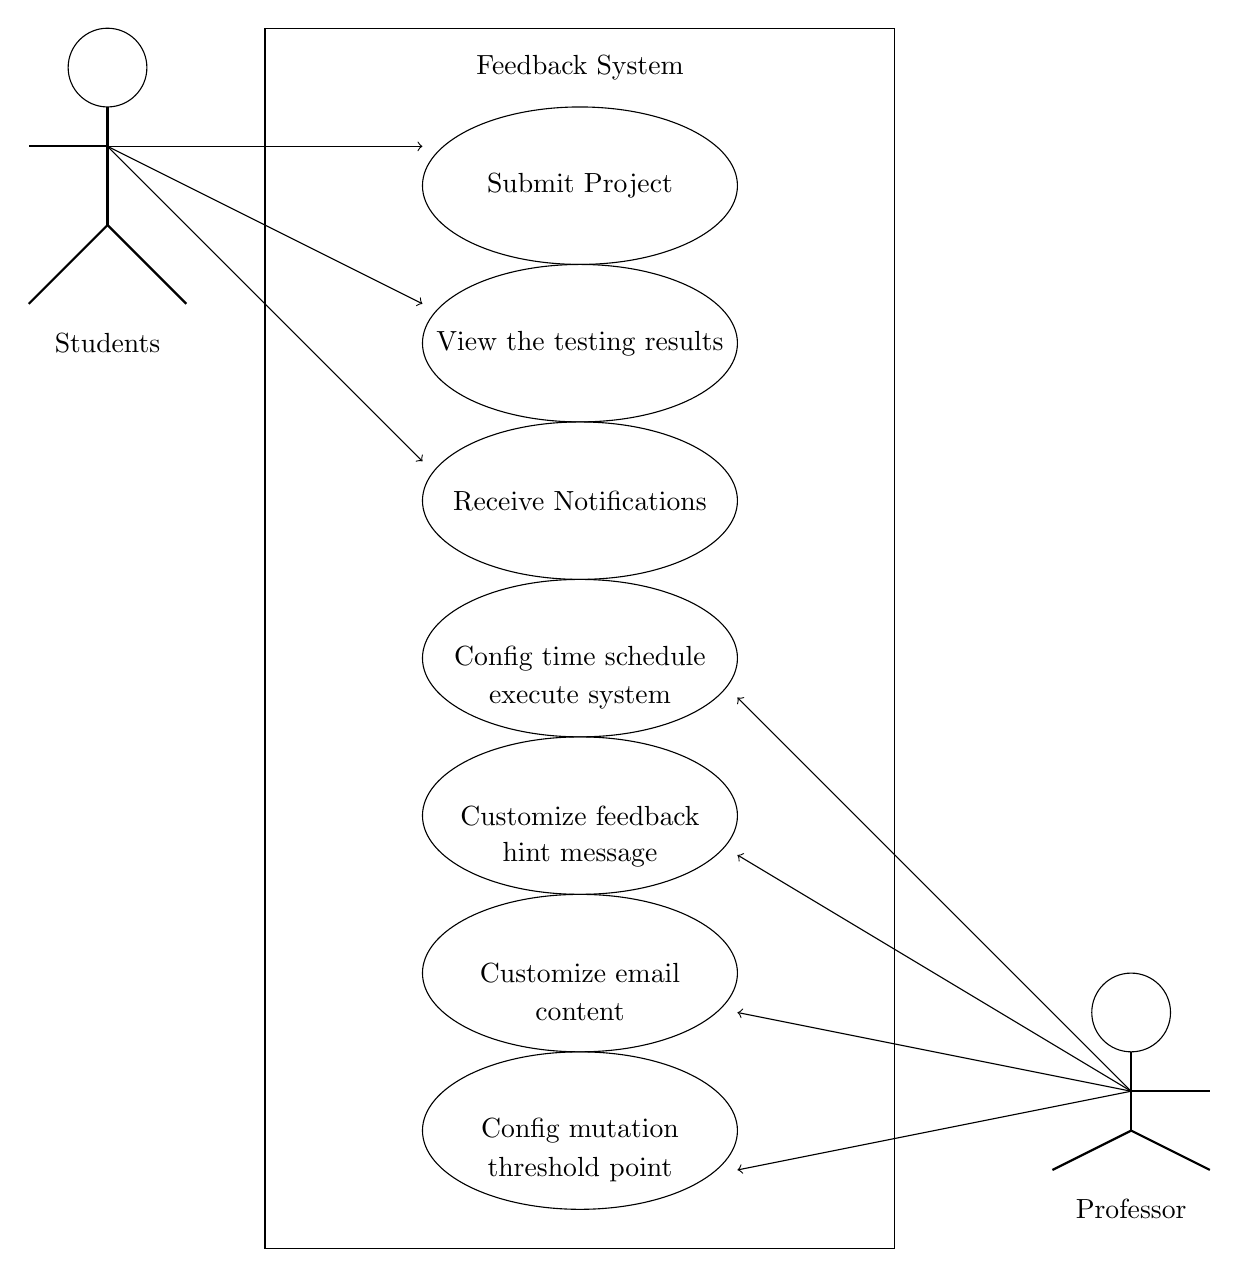
\begin{tikzpicture}
%big rectangle
\draw (0,0) rectangle (8,15.5);

%circles
\draw (4,13.5) ellipse (2cm and 1cm);
\draw (4,11.5) ellipse (2cm and 1cm);
\draw (4,9.5) ellipse (2cm and 1cm);
%\draw (5,10.5) ellipse (2cm and 1cm);

\draw (4,7.5) ellipse (2cm and 1cm);
\draw (4,5.5) ellipse (2cm and 1cm);
\draw (4,3.5) ellipse (2cm and 1cm);
\draw (4,1.5) ellipse (2cm and 1cm);

%rectangle text
\draw (4,15) node {Feedback System};

%circle text
\draw (4,13.5) node {Submit Project};
\draw (4,11.5) node  {View the testing results};
\draw (4,9.5) node {Receive Notifications};


\draw (4,7.5) node {Config time schedule};
\draw (4,7) node  {execute system};
\draw (4,5.5) node {Customize feedback};
\draw (4,5.) node {hint message};
\draw (4,3.5) node {Customize email};
\draw (4,3) node {content};
\draw (4,1.5) node {Config mutation};
\draw (4,1) node {threshold point};

%student arrows
\draw[arrows=->] (-2,14) -- (2,14); 
\draw[arrows=->] (-2,14) -- (2,12); 
\draw[arrows=->] (-2,14) -- (2,10); 

% student arms
\draw[black, thick] (-2,14.5) -- (-2,13);
\draw[black, thick] (-2,13) -- (-3,12);
\draw[black, thick] (-2,13) -- (-1,12);
\draw[black, thick] (-2,14) -- (-3,14);

%student head
\draw[color=black] (-2,15) circle (0.5cm);

\draw (-2,11.5) node {Students};

%professor arms 
\draw[black, thick] (11,1.5) -- (11,2.5);
\draw[black, thick] (11,2) -- (12,2);

%professor feet
\draw[black, thick] (11,1.5) -- (12,1);
\draw[black, thick] (11,1.5) -- (10,1);
%\draw[black, thick] (15,1.5) -- (14,2.5);

%professor head
\draw[color=black] (11,3) circle (0.5cm);

\draw (11,0.5) node {Professor};

\draw[arrows=->] (11,2) -- (6,7); 
\draw[arrows=->] (11,2) -- (6,5); 
\draw[arrows=->] (11,2) -- (6,3); 
\draw[arrows=->] (11,2) -- (6,1);


\end{tikzpicture}
\caption{Use Case Diagram}
\label{fig:f11}
\end{figure}

% \begin{figure}[h!]
% 	\centering
% 	\includegraphics[scale=0.45]{fig8.jpg}
% 	\caption{Class Diagram}
% 	\label{fig:f11}
% \end{figure}


\subsubsection{Mutation Testing Main class}
The Main class of this application will be executed first when the application executes.
\subsubsection{Properties Configuration class}
This class is used for initial configuration for the whole project. The static factory constructor from application Properties file() loads configuration from the "application.properties" file, then sets it to an instance of the Properties Configuration object.
\begin{figure}[h!]
	\centering
	\includegraphics[scale=0.90]{content/fig9.jpg}
	\caption{Properties Configuration class}
	\label{fig:f11}
\end{figure}
\subsubsection{Job Start MainFlow class}
This class is implemented from Job class, which belongs to Quartz dependency. JobStartMainFlow class is a presentation of the main flow diagram.
\begin{figure}[hb]
	\centering
	\includegraphics[scale=0.90]{content/fig10.jpg}
	\caption{Job Start Main Flow class}
	\label{fig:f11}
\end{figure}

Dependencies:
\begin{itemize}
 \item ProjectDirServiceImpl.class
\item Email ServiceImpl.class
\item Mutation Testing Service.class
\item Html Reader.class
\end{itemize}
\subsection{Project DirServiceImpl class}
This class is implemented from ProjectDirService class which provides service related to ProjectDir(submitted project dir, processing project dir, failure project dir and success project dir).
\begin{figure}[h!]
	\centering
	\includegraphics[scale=0.70]{content/fig11.jpg}
	\caption{Project DirServiceImpl class}
	\label{fig:f11}
\end{figure}
\newpage
Dependencies:
\begin{itemize}
\item Properties Configuration.class
\item Project DirService.class
\end{itemize}
\subsubsection{Email ServiceImpl class}
This class is implemented from Email Service class. This class provides service related to email actions such as send Email(), send Email With Attachments().\\
\begin{figure}[h!]
	\centering
	\includegraphics[scale=0.80]{content/fig12.jpg}
	\caption{Email ServiceImpl class}
	\label{fig:f11}
\end{figure}\\
\newpage
Dependencies:
\begin{itemize}
\item Email Service.class
\end{itemize}
\subsubsection{Mutation Testing Service.class}
This class is used for setting up and performing Junit test as well as PiTest.\\
By setting up I mean verifying the pom.xml file and injecting PiTest dependency in cases that it is not injected.
\begin{figure}[h!]
	\centering
	\includegraphics[scale=0.70]{content/fig13.jpg}
	\caption{Mutation TestingService class}
	\label{fig:f11}
\end{figure}\\
Dependencies:
\begin{itemize}
\item Modify PomXml.class
\item ProjectDirServiceImpl.class
\end{itemize}
\subsubsection{HtmlReader class}
The HtmlReader class is used to read the .html files generated by the PiTest mutation testing tool, extract the results, and write them to a file called "feedBackReport.txt" which can then be sent in an email.
\begin{figure}
	\centering
	\includegraphics[scale=0.70]{content/fig14.jpg}
	\caption{HtmlReader class}
	\label{fig:f11}
\end{figure}
\newpage
Dependencies:
\begin{itemize}
\item Mutation Sample Message Service.class
\item ProjectDirServiceImpl.class
\item PiTest Coverage Report.class
\item Feed back Message Service.class
\end{itemize}
\subsubsection{ProjectDirService class}
This is an interface that defines the methods for the ProjectDir object.
\begin{figure}[h!]
	\centering
	\includegraphics[scale=0.65]{content/fig15.jpg}
	\caption{Project DirService Interface}
	\label{fig:f11}
\end{figure}
\subsubsection{Email Service class}
This is an interface that defines the methods for the Email object.
\subsubsection{Modify PomXml.class}
This class is used to read the pom.xml file in submitted project, add PiTest dependency and PiTest plugin to that pom.xml file.\\
\\
Dependencies:
\begin{itemize}
\item InvalidProjectExeption.class
\item ProjectDirServiceImpl.class
\end{itemize}
\begin{figure}[h!]
	\centering
	\includegraphics[scale=0.70]{content/fig16.jpg}
	\caption{Modify PomXml class}
	\label{fig:f11}
\end{figure}

\subsubsection{Mutation Sample Message Service class}
This class loads the samples of mutation and the solution for each mutation operator. These files contain samples located in the “src/main/resources” directory.
\newpage
\begin{figure}[h!]
	\centering
	\includegraphics[scale=0.80]{content/fig17.jpg}
	\caption{Mutation Sample Message Service class}
	\label{fig:f11}
\end{figure}

\newpage
\begin{figure}[h!]
	\centering
	\includegraphics[scale=1.8]{content/fig18.jpg}
	\caption{Mutation Samples File}
	\label{fig:f11}
\end{figure}
\subsubsection{PiTest Coverage Report class}
This is the model class that presents PiTest coverage report object.
\newpage
\begin{figure}[h!]
	\centering
	\includegraphics[scale=0.70]{content/fig19.jpg}
	\caption{PiTest Coverage Report class model}
	\label{fig:f11}
\end{figure}

\subsubsection{Feedback Message Service class}
This class reads the file “feedback message.txt” from the “src/main/resources” directory then generates a feedback message base on the mutation result.
\newpage
\begin{figure}[h!]
	\centering
	\includegraphics[scale=0.70]{content/fig20.jpg}
	\caption{Feedback Message Service class}
	\label{fig:f11}
\end{figure}
\subsubsection{Invalid Project Exeption class}
This is a custom exception handler model.
\newpage
\begin{figure}[h!]
	\centering
	\includegraphics[scale=0.70]{content/fig21.jpg}
	\caption{Invalid Project Exception class}
	\label{fig:f11}
\end{figure}
\subsubsection{Survived Model class}
This is the model present for Survived Mutation object when executing PiTest
\begin{figure}[h!]
	\centering
	\includegraphics[width=0.40\linewidth]{content/fig22.jpg}
	\caption{Survived Model}
	\label{fig:f11}
\end{figure}

\subsubsection{FeedBack Template Parameter class}
This class declares configuration parameter mapping for the feedback file in “src/main/resources/feedback message.txt”
\begin{figure}[h!]
	\centering
	\includegraphics[scale=1.4]{content/fig23.jpg}
	\caption{Feedback Template Parameter}
	\label{fig:f11}
\end{figure}
%\newpage
\subsubsection{Mutation SamplesParamter.class}
This class declares configuration parameter mapping for mutation samples file in “src/main/resources/feedback mutation operatorName.txt”
\begin{figure}[h!]
	\centering
	\includegraphics[scale=2.6]{content/fig45.png}
	\caption{Mutation Samples Parameter}
	\label{fig:f45}
\end{figure}

\subsection{Sequence diagram}
\subsubsection{Main Sequence Diagram}
The flow diagram that illustrates the steps and stages that must be followed in order for a solution to be submitted to the feedback system.\par 
% \begin{figure}[h!]
% 	\centering
% 	\includegraphics[scale=0.25]{content/fig24.jpg}
% 	\caption{Main sequence diagram}
% 	\label{fig:f11}
% \end{figure}
The above flow diagram illustrates the main functionalities of the Mutation Testing System. The Main class of this application will be executed first when the application executes. It starts with the Main function which trigger a scheduler, as well as loading cron expressions from an application properties file. The scheduler then invokes the Job Start MainFlow function.\par 
The Job Start MainFlow function first calls IsHaveNewProjectSubmitted() method on the Project DirServicelmpl class to check whether there are any new projects in the ‘submitted project’ folder. If there are no new projects, it will console log a description and wait for the next scheduled time. Otherwise, it will call getListProject() method on Project DirServicelmpl class to get an array of project names. \par 
It will then loop through these project names and check if each project name is invalid or not. If it is found to be invalid, it will call move Project From Submitted ToFailureDir() method on Project DirServicelmpl class to move this project from the submitted directory to a failure directory. Otherwise, it will call setup Selected Project And Perform Testing() on Mutation Testing Service to set up and perform unit tests and PiTest on the project before receiving a response if the test has been completed successfully or not from Mutation Testing Service class. \par 
If it has been completed successfully, Job Start MainFlow will call show Report() method on HtmlReader class to read the mutation testing results before sending an email notification about the results of these tests via send Email() method on Email Servicelmpl class. 

Finally, depending on whether or not the mutation testing is passed, JobStartMainFlow method will either call move Project To SuccessDir() method or move Project ToFailureDir() method on Project DirSErvicelmpl class before looping through any remaining projects in its array until all have been tested.

\subsubsection{Junit test Sequence Diagram}
In the main flow diagram, mutation testing service sets up and performs unit tests and PiTest on the project before receiving a response if the test has been completed successfully or not
\par
There are five steps that are followed in order to complete the process of Junit test which are triggered by the main flow that is shown in the flow diagram below.\par 
% \begin{figure}[h!]
% 	\centering
% 	\includegraphics[scale=0.35]{content/fig25.jpg}
% 	\caption{Junit test sequence diagram}
% 	\label{fig:f11}
% \end{figure}
The above Junit test and PiTest flow starts with the Job StartMainFlow function, which calls setupSelected Project Testing() method on Mutation Testing Service class to set up and perform unit tests and mutation tests on the project. This process begins by calling create Commands For Unit Testing With full ProjectPath() method on Mutation Testing Service class to create commands for unit testing. Then, the write CommandToFile() method is called to write the command to a file. After that, perform JUnitTesting Process Builder() method is called to execute the unit test. If the unit test fails, it will return false, otherwise it will move to the next step of executing mutation test.

\subsubsection{PiTest Sequence Diagram}
This diagram shows where you can find the auto generated PiTest feedback report.\par 
% \begin{figure}[h!]
% 	\centering
% 	\includegraphics[scale=0.45]{content/fig26.jpg}
% 	\caption{PiTest sequence diagram}
% 	\label{fig:f11}
% \end{figure}
The MutationTestingService provides a way for students to obtain feedback on their code quality in a timely manner. This is achieved by first including the PiTest dependency in the pom.xml file of the project. In order to do this, the ModifiedModelToFileWithFullProjectPath() method is used to write the PiTest dependency into the pom.xml file in ModifyPomXml.PopulateModifiedModelWithFullProjectPath() method then parses the pom.xml file into a model object and adds both the PiTestDependency() and Plugin(). These are then returned back to MutationTestingService class for further processing.\par 

Once returned, createCommandsForMutationTestingWithFullProjectPath() method is called to create commands for mutation testing and perform mutation testing using ProcessBuilder() method to execute the mutation test before returning true if successful and false if unsuccessful. Through this process, students can receive feedback on their projects based on the results of these tests and make necessary changes accordingly in order to improve their code quality.
\begin{figure}[h!]
	\centering
	\includegraphics[scale=0.8]{content/fig27.jpg}
	\caption{PiTest report}
	\label{fig:f11}
\end{figure}
\newpage
\subsubsection{Extract report flow}
  [As discussed in the MAIN FLOW DIAGRAM, if the response has been completed successfully, Job Start Main Flow will call show Report() on Html Reader to read the mutation testing results.] \\
% \begin{figure}[h!]
% 	\centering
% 	\includegraphics[scale=0.45]{content/fig28.jpg}
% 	\caption{Extract report}
% 	\label{fig:f11}
% \end{figure}
% \newpage
The extract report flow begins with the JobStartMainFlow function, which calls ShowReport() method on HtmlReader to read the mutation testing results. After reading the HTML files, HtmlReader extracts the report and stores it in the PiTestCoverageReport model. It also reads and prints the report details to a file named “feedbackReport.txt”.\par
The response of the testing is then sent back to JobStartMainFlow. Subsequently, JobStartMainFlow triggers an email notification about the results of these tests through SendAttachmentEmail() method, attaching the “feedbackReport.txt” file to EmailServicelmpl class.\par 
Depending on whether or not the mutation testing passed, JobStartMainFlow will either call moveProjectToFailureDir() method on EmailServicelmpl class or moveProjectToSuccessDir() method on ProjectDirServicelmpl class before looping through any remaining projects in its array until all of them have been tested. This ensures that students receive accurate feedback about their projects in a timely manner.
\subsubsection{Unit test cases}
JUnit library is used to create unit test cases. Three test classes were added to cover unit testing of all logic parts in the application. These three classes are available in the package com.mutation.service under the folder src/test/java.
\subsection{Maven library}
Maven library added to the application is to execute JUnit testing and PiTesting of the submitted project.
%\newpage
\begin{figure}[h!]
	\centering
	\includegraphics[scale=0.70]{content/fig29.jpg}
	\caption{maven library}
	\label{fig:f11}
\end{figure}
\subsection{Folders}
\subsubsection{Submitted Folder}
This is a local folder, which store student submitted projects. This project synced with the Dropbox submitted projects folder.\\
The dir path config in application.properties files.
\begin{figure}[h!]
	\centering
	\includegraphics[scale=0.52]{content/fig30.jpg}
	\caption{Submitted folder configuration}
	\label{fig:f11}
\end{figure}
\newpage
\subsubsection{Project Processing}
This is a local folder that stores student projects while they are being tested. The dir path config in application.properties files.
\begin{figure}[h!]
	\centering
	\includegraphics[scale=0.52]{content/fig31.jpg}
	\caption{Project Processing folder configuration}
	\label{fig:f11}
\end{figure}
\subsubsection{Project Success}
This is a local folder that stores student projects that are tested and pass both the Junit test and PiTest coverage threshold.\\
The dir path config in application.properties files.
\begin{figure}[h!]
	\centering
	\includegraphics[scale=0.52]{content/fig32.jpg}
	\caption{Project Success folder configuration}
	\label{fig:f11}
\end{figure}
\subsubsection{Project Failure}
This is a local folder that stores student projects that are tested and do not pass the Junit test or PiTest coverage threshold.\\
The dir path config in application.properties files.
 \begin{figure}[h!]
	\centering
	\includegraphics[scale=0.91]{content/fig33.png}
	\caption{Project Failure folder configuration}
	\label{fig:f11}
\end{figure}

\subsection{Application properties file}
Application.properties file is added in the project where the professor can set the threshold value of mutation coverage percentage.
\newpage
\begin{figure}[h!]
	\centering
	\includegraphics[scale=1]{fig34.png}
	\caption{Application properties file}
	\label{fig:f11}
\end{figure}
\subsection{Resources}
\subsubsection{Feedback message.txt.}
A template for a feedback message is found in the file feedback message.txt, which is kept in the resources folder. Using this template, a unique feedback message regarding the PiTest report's survivor mutants is created and delivered to the student as part of their feedback report.
\begin{figure}[h!]
	\centering
	\includegraphics[scale=1]{fig35.png}
	\caption{Feedback Message file}
	\label{fig:f11}
\end{figure}
\newpage
\subsubsection{Feedback mutation sample.txt.}
The feedback mutation sample.txt file is also included in the resources folder.
\begin{figure}[h!]
	\centering
	\includegraphics[scale=1.3]{fig36.png}
	\caption{Mutation Samples file}
	\label{fig:f11}
\end{figure}
\newpage
\subsection{Email project tested body.txt}
The body of email notification to students when the submitted project is tested could be a failure or success to pass the testing threshold.
\begin{figure}[h!]
	\centering
	\includegraphics[scale=1.3]{fig37.png}
	\caption{Email project tested body}
	\label{fig:f11}
\end{figure}

\newpage
\subsubsection{Email project not tested body.txt}
The body of email notification to students when the submitted project is not tested could be the wrong project format name, or the project does not have a pom.xml file.\\


Dear <StudentName>\\
I am pleased to inform you that your project has been tested. Depending on the results of the testing, I have the following feedback for you:\\

\textbf{Body 1$:$ Project Not Tested$:$} The project had been scanned; however, it was not tested due to <the reason>. Please check the project in the folder 'project\_not\_tested' on Dropbox and resubmit it after you have fixed any issues. \\
\newpage
\begin{figure}[h!]
	\centering
	\includegraphics[scale=1.3]{fig37.png}
	\caption{Email project\_tested\_body.txt}
	\label{fig:f11}
\end{figure}\\
\textbf{Body 2$:$ Project Tested but Failed at Unit Testing$:$} The project had been scanned and tested but there are some test cases that failed. <List test case failed>. Please update these test cases and resubmit them. \\
\begin{figure}[h!]
	\centering
	\includegraphics[scale=1.9]{content/Figure-3.34_new_-Email-project-not-pass-unit-test-body.jpg}
	\caption{Email project\_not\_pass\_unit\_test\_body.txt}
	\label{fig:f11}
 %Email project tested body
\end{figure}\\
\textbf{Body 3$:$ Project Tested but Failed at Mutation Testing$:$} The project had been scanned and tested but the test case is not good enough. You need to improve the test case to make it better. Please read the attached file 'feedBackReport.txt' for further details regarding how to improve the test case.\\
\begin{figure}[h!]
	\centering
	\includegraphics[scale=1.9]{content/Figure-3.35_new_-Email-project-not-pass-mutation-body.jpg}
	\caption{Email project\_not\_pass\_mutation\_body.txt}
	\label{fig:f11}
\end{figure}\\
\newpage
\textbf{Body 4$:$ Project Tested and Successful$:$} Congratulations! The project has passed all checks and been successfully tested. Well done and keep up the good work!\\
If you have any questions or would like further clarification, please do not hesitate to contact me directly or via email. \\
\begin{figure}[h!]
	\centering
	\includegraphics[scale= 1.9]{content/Figure-3.36_new_-Email-project-passed-body.jpg}
	\caption{Email project\_passed\_body.txt}
	\label{fig:f11}
\end{figure}\\
Regards,\\
$[$Professor Email Signature$]$ \\ 


\newpage
Project format name: \\ 
Mr.StudenName\_ProjectName\_Email\_yyymmddHHMM\\
Mrs.StudenName\_ProjectName\_Email\_yyymmddHHMM
%Mr.StudenName_ProjectName_Email_yyymmddHHMM 
%Mrs.StudenName_ProjectName_Email_yyymmddHHMM
\newline

Project name Restriction: \\ 
The length of the project name is can be only between 1 to 40 characters\\
\newline
Example of project name: 
%\\Mr.studiName_BankingApplicationSystem_anhnd6893@gmail.com_202301091803
\\Mr.studiName\_BankingApplicationSystem\_anhnd6893@gmail.com\_202301091803
%\newline
%   \begin{figure}[h!]
% 	\centering
% 	\includegraphics[scale=1.1]{content/Figure-3.30_new_-Project-Invalid-Name-config.jpg}
% 	\caption{Projects\_invalid\_name}
% 	\label{fig:f11}
% \end{figure}
\subsection{Feedback report}
\subsubsection{PiTest generated report}
After executing the PiTest, the mutation test report named “PiTest-reports” will be generated in the folder name “target” of the project being tested.\par 
Example: \\%StudentBankingAppAssignment_kontaktlourenz@yahoo.de_202301070608\target\PiTest-reports
StudentBankingAppAssignment\_kontaktlourenz@yahoo.de\_202301070608\textbackslash{}target\textbackslash{}PiTest-reports
%\newpage
\begin{figure}[h!]
	\centering
	\includegraphics[scale=0.70]{content/fig39.jpg}
	\caption{PiTest report location}
	\label{fig:f11}
\end{figure}

It contains a list of mutation test history folders named in the format year-date-month-hour-mins.\\
Example: 202301071958
\newpage
\begin{figure}[h!]
	\centering
	\includegraphics[scale=0.70]{content/fig40.jpg}
	\caption{PiTest report history}
	\label{fig:f11}
\end{figure}
%\newpage
The detail of the PiTest is in the html file.
\begin{figure}[h!]
	\centering
	\includegraphics[scale=0.70]{content/fig41.jpg}
	\caption{PiTest report detail location}
	\label{fig:f11}
\end{figure}
\newpage
\begin{figure}[h!]
	\centering
	\includegraphics[scale=0.70]{content/fig42.jpg}
	\caption{PiTest report detail}
	\label{fig:f11}
\end{figure}
\newpage
\subsubsection{Feedback message report}
The feedback message report file name “feedBack Report.txt” generated in the folder name “target” of the project being tested.\\
Example: \\%StudentBankingAppAssignment_kontaktlourenz@yahoo.de_202301070608\target\feedBackReport.txt
StudentBankingAppAssignment\_kontaktlourenz@yahoo.de\_202301070608\textbackslash{}target\textbackslash{}feedBackReport.tx
\begin{figure}[h!]
	\centering
	\includegraphics[scale=0.75]{content/fig43.jpg}
	\caption{Feedback report file}
	\label{fig:f11}
\end{figure}

\begin{figure}[h!]
	\centering
	\includegraphics[scale=0.75]{content/fig44.jpg}
	\caption{A part of Feedback report content}
	\label{fig:f11}
\end{figure}



%\noindent\lipsum[10-15]

